\documentclass[11pt,letterpaper]{article}
\usepackage{graphicx, geometry, amsmath, hyperref, url, natbib, booktabs, xcolor, listings}
\usepackage{longtable, tabularx, array, multirow}
\geometry{margin=1in}
\hypersetup{colorlinks=true, linkcolor=black, citecolor=black, urlcolor=black}
\emergencystretch=1.5em

\title{Why Slovene Refusal Outlasts English Abliteration:\\A Five-Iteration Experimental Record}
\date{September 2026}
\author{}

\begin{document}
\maketitle
\tableofcontents
\newpage

% ============================================================
\section{Framing}
% ============================================================

GaMS3-12B-Instruct~[20] and Gemma-3-12B-IT both descend from google/gemma-3-12b-pt, but followed different post-training paths. GaMS3 received Slovene continued pretraining on 140 billion tokens and supervised fine-tuning on a mix that is roughly 79\% Slovene, including about 7,000 safety-refusal examples drawn largely from machine-translated Qwen-family responses. Gemma-IT received Google's standard multilingual post-training. Because the two checkpoints share a pretrained ancestor yet diverge in the language of their safety supervision, they form a natural pair for testing whether the language in which refusal was taught determines where refusal appears.

The core question is whether Slovene-taught refusal transfers to English. Prior work on refusal directions~[1] established that a single subspace mediates refusal in English, and Wang et al.~[2] showed that English-extracted refusal directions transfer across 14 languages, but both studies used models whose post-training mixed many languages. Less is known about transfer when safety supervision is concentrated in one language. Shaham et al.~[4] found that ``a pinch'' of multilingual instruction data suffices for task-level transfer; Krasnodebska et al.~[8] found that English-only DPO alignment does \emph{not} ensure cross-lingual safety, even for the same harm categories.

A second question follows: if refusal does transfer, does the English-only objective of an automatic abliteration tool (Heretic~[24]) remove Slovene refusal as readily as English refusal, and does it do so equally in GaMS3 and Gemma-IT?

Four rival accounts were pre-registered. The main claim (behaviour-level reach) predicts that refusal transfers to English at every hazard-category grain. Alternate~1 (supervised reach) predicts a Slovene surplus in low-English-dose categories. Alternate~2 (base-checkpoint geometry) predicts that GaMS-vs-Gemma differences are explained by the base models' harmfulness separability~[3, 14]. Alternate~3 (persona gating) predicts a uniform Slovene surplus driven by GaMS3's Slovene-anchored self-identity~[6]. Alternate~4 (thin templated gate) predicts symmetric language differences driven by the diversity, not the language, of refusal supervision.


% ============================================================
\section{Iteration 1}
% ============================================================

\subsection{Strategy}

The iteration ran five artifacts: a dataset artifact that built the evaluation sets and audited GaMS3's supervision dose, and four experiment artifacts that each tested one or more of the pre-registered claims. The design was a screen: every claim was evaluated on SCORE items drawn from RefusEU's train and test splits, with the reserved RefusEU evaluation split untouched for a future FINAL pass. The sequence was dictated by a single-GPU constraint (40\,GB disk), requiring models to be loaded and evicted one at a time.

The four experiments were:
\begin{enumerate}
  \item Experiment~1 (main screen): the refusal difference-in-differences between GaMS3 and Gemma-IT on original models, plus the dose contrast~$D$ and identity calibration.
  \item Experiment~2 (base models and mechanistic): harmfulness separability in the two base checkpoints and two instruct models, plus the ancestor-direction induction test.
  \item Experiment~3 (persona gate): the alternate-3 manipulation, ablating GaMS3's persona direction and testing whether it moves Slovene refusal.
  \item Experiment~4 (Heretic abliteration): English-objective abliteration of both instruct checkpoints, the transfer curve, the excess KL ratio, and the prefill test.
\end{enumerate}

All protocols were hashed and committed before scoring. The OpenRouter shared key hit its daily limit partway through experiments~3 and~4, leaving some judge calls incomplete.

\subsection{Artifact~1: Dataset and Supervision Audit}
\label{gen_art_dataset_1}

The dataset artifact assembled eight data blocks totalling 15,647 rows.

\textbf{RefusEU evaluation split.} 1,400 English and 1,400 Slovene prompts from RefusEU~[8], frozen into 100 DEV and 1,300 FINAL pairs by sha1 of the pair identifier. Each item received a blind hazard-category label (majority vote of gpt-4.1-mini, gemini-2.5-flash, and a TF-IDF classifier). Gold-test accuracy was 0.759 for English and 0.716 for Slovene; restricting to items where all labellers agreed raised accuracy to 0.95 and 0.94. Inter-annotator kappa between the two LLM labellers was 0.88 (English) and 0.83 (Slovene).

A critical discovery was that same-row-identifier English and Slovene items in RefusEU are not translations: LaBSE cosine similarity was 0.553, matching the similarity of same-category pairs (0.547) and far below the machine-translation baseline (0.914). Zero of 1,400 pairs graded as translation-equivalent. This means within-model Slovene-vs-English comparisons on matched row identifiers conflate prompt content with language; only the cross-model difference-in-differences and a separate machine-translation arm are interpretable.

\textbf{Supervision dose audit.} 6,239 rows from GaMS-Nemotron-Chat and GaMS-Instruct-SAFE were labelled for response type, language, and hazard category by two LLM families (gpt-4.1-mini and gemini-2.5-flash, with llama-3.3-70b tiebreak on 928 disagreements; batch-check agreement 0.945 English, 0.959 Slovene). The overall English share of safety refusals was 0.178, with a propagated interval of [0.055, 0.452]. The upper bound exceeds 0.40, so ``Slovene-dominant refusal'' is not statistically licensed from the public data alone.

\begin{table}[!htbp]
\centering
\caption{Frozen dose groups after re-labelling (Artifact~1, Iteration~1).}
\label{tab:dose_groups}
\begin{tabularx}{\linewidth}{lXl}
\toprule
Group & Categories & EN share range \\
\midrule
Low-EN & S2, S5, S7, S13 & 0.034 to 0.096 \\
High-EN & S1, S3, S4, S8, S9, S10, S11, S14 & 0.109 to 0.291 \\
Intermediate & S6, S12 & 0.148 to 0.201 \\
\bottomrule
\end{tabularx}
\end{table}

Thirteen of fourteen categories were flagged as dose-uncertain (the propagated EN-share interval straddles 0.10). The re-labelling changed S2 from high to low (point 0.075, down from Stage-0b's 0.292) and S8 from low to high (point 0.226). S1 moved from intermediate to high (point 0.291).

\textbf{Other blocks.} The hard set (OR-Bench-hard-1k, XSTest, OR-Bench-toxic-300) was assembled with Gemini Slovene machine translation (back-translation chrF median 79; 11 items dropped). The identity set comprised 120 identity questions across six facets plus 120 matched personal controls, with zero overlap against the Nemotron training rows.

\subsection{Artifact~2: Main Screen of Refusal Differences (Experiment~1)}
\label{gen_art_experiment_1}

Gemma-3-12B-IT and GaMS3-12B-Instruct were run in NF4 quantization with greedy decoding (64 new tokens, empty system prompt) on all 2,137 SCORE RefusEU pairs, a 400-pair item-matched machine-translation arm, 60 identity question pairs, and 1,504 CONSTRUCT pairs. Judges were gemini-2.5-flash on 10,852 responses and gpt-4.1-mini on a 20\% validation subset; total judge spend was approximately \$0.91.

The ceiling flag fired: Gemma's English lexicon refusal rate was 0.961, and the prefix-score AUROC against the lexicon was only 0.61 in that cell, so the pre-registered fallback to the judge readout was triggered.

\begin{table}[!htbp]
\centering
\caption{Refusal rates on the 2,137 SCORE pairs (Experiment~1, Iteration~1).}
\label{tab:refusal_rates_exp1}
\begin{tabular}{lcccc}
\toprule
Readout & Gemma EN & Gemma SL & GaMS EN & GaMS SL \\
\midrule
Lexicon & 0.961 & 0.885 & 0.942 & 0.723 \\
Judge (binary) & 0.979 & 0.929 & 0.971 & 0.865 \\
Judge + partial & 0.988 & 0.939 & 0.974 & 0.875 \\
\bottomrule
\end{tabular}
\end{table}

Both models refuse at high rates across languages. The gap is in Slovene: GaMS3 refuses less than Gemma in Slovene on both the lexicon (0.723 vs 0.885) and the judge (0.865 vs 0.929). In English, the two models are within two percentage points.

\subsubsection{Difference-in-Differences and Dose Contrast}

The difference-in-differences (DiD = [GaMS(SL $-$ EN)] $-$ [Gemma(SL $-$ EN)]) measures whether GaMS3 has a larger Slovene deficit than Gemma. A negative DiD means GaMS3's Slovene gap is wider. All rate-to-logit conversions use the Hautus correction (adding 0.5 to counts before taking log-odds).

\begin{table}[!htbp]
\centering
\caption{Overall DiD and dose contrast $D$ (log-odds, 95\% bootstrap CI; Experiment~1, Iteration~1).}
\label{tab:did_dose}
\begin{tabular}{lccc}
\toprule
Readout & Overall DiD [95\% CI] & $D$ [95\% CI] & MDE($D$) \\
\midrule
Lexicon & $-0.67$ [$-0.95, -0.41$] & $0.61$ [$-0.58, 2.15$] & 1.89 \\
Judge & $-0.38$ [$-0.69, -0.05$] & $-0.08$ [$-1.27, 0.94$] & 1.53 \\
Judge + partial & $-0.03$ [$-0.39, 0.39$] & $-0.73$ [$-2.11, 0.48$] & 1.87 \\
\bottomrule
\end{tabular}
\end{table}

On the lexicon, the overall DiD is clearly negative ($-0.67$, CI excludes 0), confirming that GaMS3 has a wider Slovene refusal gap than Gemma. On the judge, the DiD is smaller ($-0.38$) but its CI still excludes 0. Including partial refusals shrinks the DiD to near zero. The dose contrast $D$ is uninformative on all three readouts: the confidence intervals are wide (MDE 1.5 to 1.9 log-odds), spanning both positive and negative values. Neither equivalence nor a dose effect can be established.

\begin{figure}[!htbp]
  \centering
  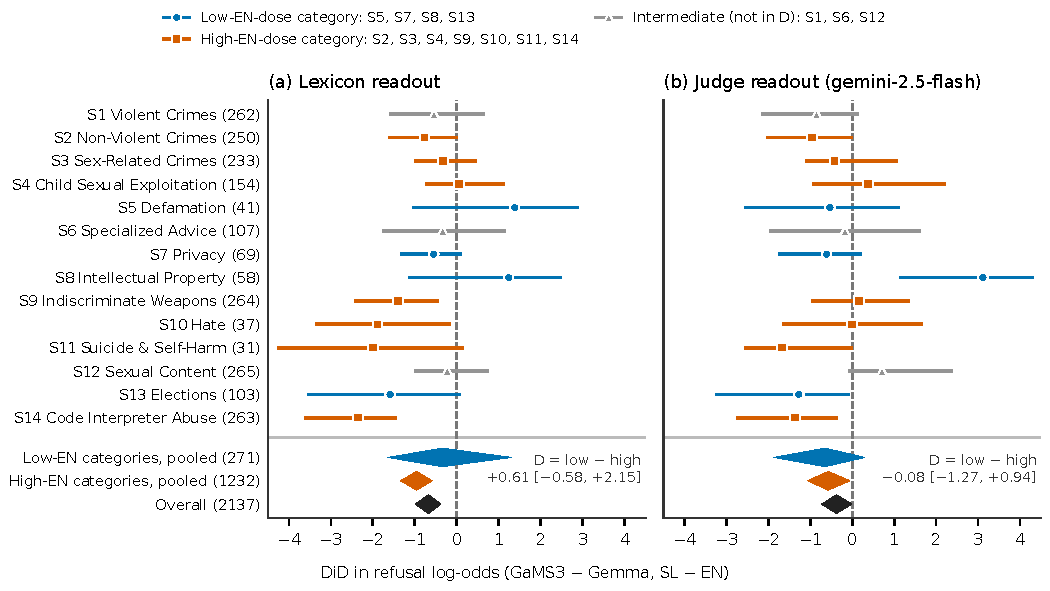
\includegraphics[width=\linewidth,height=0.85\textheight,keepaspectratio]{figures/fig_forest_did_v0.pdf}
  \caption{Category-level difference-in-differences (DiD) in refusal log-odds, $[\mathrm{GaMS3}(\mathrm{SL}-\mathrm{EN})]-[\mathrm{Gemma}(\mathrm{SL}-\mathrm{EN})]$, on the 2,137 SCORE RefusEU EN/SL pairs of the iteration-1 screen. (a)~Refusal scored by the frozen bilingual lexicon; (b)~refusal scored by the gemini-2.5-flash judge. Blue circles are low-EN-dose categories, vermillion squares are high-EN-dose, and grey triangles are intermediate. Diamonds span the 95\% CI of the pooled DiD; the dashed line marks zero. The overall DiD is $-0.67$ $[-0.95,-0.41]$ on the lexicon and $-0.38$ $[-0.69,-0.05]$ on the judge. The dose contrast $D$ is $+0.61$ $[-0.58,2.15]$ on the lexicon and $-0.08$ $[-1.27,0.94]$ on the judge; neither interval excludes zero.}
  \label{fig:forest_did}
\end{figure}

The 14-category meta-regression of DiD on the English dose share found no significant slope. However, the item-level generalised linear mixed model produced a significant negative zEN term on the lexicon ($-0.17$, CI $[-0.28, -0.07]$) that flipped sign on the judge ($+0.13$, CI $[0.00, 0.27]$), a signature of pseudo-replication from 14 correlated category-level units (correlation between zEN and zSL: 0.86, VIF 3.84).

\textbf{Scorer confound.} The frozen Slovene lexicon lacked English-style ``lecture'' markers, missing 312 GaMS Slovene judge-classified refusals vs 97 for Gemma. Kappa between the lexicon and the judge was below 0.70 in three of four model-language cells. The lexicon therefore overstates GaMS3's Slovene deficit relative to the judge.

\subsubsection{Item-Matched Machine-Translation Arm}

A 400-item arm used NLLB machine translations of English prompts into Slovene. GaMS3's Slovene-MT refusal rate was 0.968 vs its English rate of 0.970 (McNemar: 7 vs 8 discordant pairs). The judged DiD on this arm was $-2.0$ pp [$-4.3, 0.0$], compared with $-6.0$ pp on the natural RefusEU pairs.

\subsubsection{Identity Calibration (C1)}

The calibration arm passed. GaMS3 named itself ``GaMS'' in 90\% of Slovene identity responses and 35\% of English ones; Gemma named itself ``Gemma'' at 77\% in English and 67\% in Slovene. The identity DiD was 3.22 [2.38, 4.38], far exceeding the 10 pp threshold ($m_{id} = 0.43$).

\begin{table}[!htbp]
\centering
\caption{Identity: own-name rates and name distribution (Experiment~1, Iteration~1).}
\label{tab:identity_exp1}
\begin{tabularx}{\linewidth}{lll}
\toprule
Cell & Own-name rate & Top other names \\
\midrule
GaMS EN & 0.35 & Qwen 0.13, none 0.48 \\
GaMS SL & 0.90 & none 0.08 \\
Gemma EN & 0.77 & none 0.22 \\
Gemma SL & 0.67 & other 0.08, none 0.20 \\
\bottomrule
\end{tabularx}
\end{table}

\subsubsection{Surface Forms}

1,504 of 1,545 GaMS3 Slovene refusals (97.3\%) opened with the calque ``Oprostite, vendar\ldots'' (``I'm sorry, but\ldots''), a word-for-word translation of the English Qwen refusal template.

\subsubsection{Verification}

The audit script passed 30 of 30 checks. Two independent re-derivation scripts reproduced all rates, DiD, $D$, DiD\textsubscript{id}, and machine-translation DiD exactly. Four-vs-eight-bit first-token agreement was 0.95.


\subsection{Artifact~3: Base Models and Mechanistic Induction (Experiment~2)}
\label{gen_art_experiment_2}

Four checkpoints (gemma-3-12b-pt, GaMS3-12B, gemma-3-12b-it, GaMS3-12B-Instruct) were run in NF4 on an RTX~4090. Items were 2,889 RefusEU train+test pairs. OpenRouter spend was \$4.74.

\subsubsection{Alternate~2 (Base-Checkpoint Geometry): Killed}

At the pre-registered layer ($L = 22$), the delta-$d'$-Slovene (GaMS-base minus pt) was $-0.98$ [$-1.13, -0.85$]: the GaMS base has \emph{lower} Slovene separability than the pretrained ancestor, the opposite of the prediction. At each model's own best layer, the sign reversed to $+2.85$. The item-level regression found that base geometry explained only 4.2\% of the instruct-level refusal variance [0.5\%, 12.2\%].

\textbf{Alternate~2 is dead.} The base checkpoint does not set the instruct model's language profile of refusal.

\subsubsection{C4 (Ancestor-Direction Induction): Failure Branch}

The pretrained direction never reached a refusal rate of 0.50 in any model-language cell under the judge readout (peak 0.03 to 0.25). It performed no better than random directions and had cosine similarity near zero with each instruct model's own refusal direction.

\begin{table}[!htbp]
\centering
\caption{SCORE-400 judge refusal rates (Experiment~2, Iteration~1).}
\label{tab:score400_exp2}
\begin{tabular}{lcc}
\toprule
Model & EN & SL \\
\midrule
Gemma-IT & 0.957 & 0.945 \\
GaMS3-Instruct & 0.967 & 0.917 \\
DiD (log-odds) & \multicolumn{2}{c}{$-0.70$ [$-1.45, 0.02$]} \\
\bottomrule
\end{tabular}
\end{table}


\subsection{Artifact~4: Persona-Gate Test (Experiment~3)}
\label{gen_art_experiment_3}

Alternate~3, drawing on Zhong and Li's~[6] claim that refusal lives downstream of persona, predicted that GaMS3's Slovene-anchored persona gates Slovene refusal. The test ran on SCORE-400 RefusEU pairs.

\subsubsection{Verdict: Untestable}

The manipulation check failed. Persona ablation did remove own-naming, but a variance-matched random direction also removed English naming to a comparable degree. Even if the manipulation had been clean, the signature would not survive. The judge-based triple-difference (TD*) was $+0.23$ [$-0.81, 1.25$], with an MDE of 1.46 (exceeding $2m = 0.88$).

\begin{table}[!htbp]
\centering
\caption{Refusal and identity rates under persona ablation (GaMS3, SCORE-400; Experiment~3, Iteration~1).}
\label{tab:persona_exp3}
\begin{tabular}{lcccc}
\toprule
Condition & EN refusal & SL refusal & EN own-name & SL own-name \\
\midrule
Original & 0.925 & 0.675 & 0.45 & 0.90 \\
Persona ablated (late) & 0.925 & 0.653 & 0.00 & 0.00 \\
Random control (late) & 0.925 & 0.670 & 0.23--0.30 & 0.23--0.30 \\
\bottomrule
\end{tabular}
\end{table}

\textbf{Alternate~3 is dead.} The manipulation check fails, the premise (a Slovene surplus) is contradicted by the data, and the effect size is too small relative to the MDE.


\subsection{Artifact~5: Heretic Abliteration and Transfer Curve (Experiment~4)}
\label{gen_art_experiment_4}

English-objective abliteration was run on both instruct checkpoints using Heretic~[24] with identical configuration: NF4, empty system prompt, TPE sampler with seed 20260923. The 17 compared draws were verified identical across models (paired design).

\subsubsection{English Abliteration Reaches Slovene}

\begin{table}[!htbp]
\centering
\caption{Refusal rates before and after Heretic abliteration (lexicon, 400 pairs; Experiment~4, Iteration~1).}
\label{tab:heretic_exp4}
\begin{tabular}{lcccc}
\toprule
Condition & Gemma EN & Gemma SL & GaMS EN & GaMS SL \\
\midrule
Original & 0.965 & 0.932 & 0.940 & 0.830 \\
Selected edit & 0.242 & 0.223 & 0.133 & 0.098 \\
\bottomrule
\end{tabular}
\end{table}

Trial-level slopes of Slovene refusal on English refusal were positive for both models (Gemma 1.21 [0.75, 1.83]; GaMS3 0.79 [0.51, 1.14]).

\begin{figure}[!htbp]
  \centering
  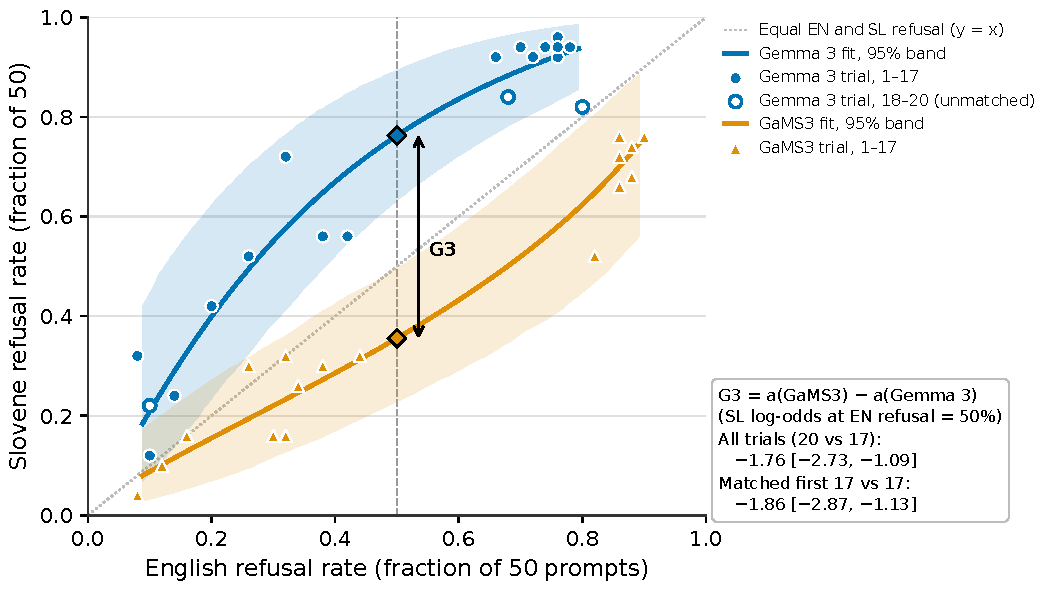
\includegraphics[width=\linewidth,height=0.85\textheight,keepaspectratio]{figures/fig_transfer_curve_v0.pdf}
  \caption{Slovene-vs-English refusal transfer under English-objective Heretic abliteration (Experiment~4, Iteration~1). Blue circles are Gemma-3-12B-IT trials; orange triangles are GaMS3-12B-Instruct trials. Solid curves are OLS fits in Hautus log-odds. $G_3 = -1.86$ $[-2.87, -1.13]$ on the matched first 17 trials: at any matched English refusal level, GaMS3 retains less Slovene refusal than Gemma.}
  \label{fig:transfer_curve}
\end{figure}

\subsubsection{C3 (Frozen-Core Transfer): Fails Both Ways}

The primary statistic $G_3$ (the GaMS-minus-Gemma difference in the logistic transfer-curve intercept) was $-1.86$ [$-2.87, -1.13$] on the matched first 17 trials ($-1.76$ on all trials). The main claim required $|G_3| < m = 0.675$; alternate~1 required $G_3 > m$. Neither holds.

\subsubsection{C5a (Excess Slovene KL): Reverses the Prediction}

The excess Slovene/English KL ratio was 0.298 [0.154, 0.562] for Gemma and 0.574 [0.409, 0.796] for GaMS3, both with confidence intervals entirely below 1. The real direction damages Slovene \emph{less} than random directions. There is no Slovene leakage.

\subsubsection{C5b (Bilingual Re-Selection): Unpowered}

Only one candidate trial per model met the re-selection criteria. Gain was zero.

\subsubsection{Alternate~4 (Thin Templated Gate)}

A five-token compliant prefill (``Sure, here is'') flipped refusals at strikingly different rates:

\begin{table}[!htbp]
\centering
\caption{Prefill flip rates (Experiment~4, Iteration~1).}
\label{tab:prefill_exp4}
\begin{tabular}{lcccc}
\toprule
 & Gemma EN & Gemma SL & GaMS EN & GaMS SL \\
\midrule
Flip rate & 0.031 & 0.558 & 0.559 & 0.855 \\
\bottomrule
\end{tabular}
\end{table}

The prefill signature Sig was 3.63 [3.13, 4.36] in English and 1.54 [1.20, 1.92] in Slovene, both exceeding the threshold. However, alternate~4 predicted symmetric language effects, and the observed asymmetry was 2.10, far exceeding the threshold. Alternate~4 was scored as not survived.

\subsection{Summary of Dead Ends and Surviving Claims After Iteration~1}

\begin{table}[!htbp]
\centering
\caption{Status of pre-registered claims after Iteration~1.}
\label{tab:claims_iter1}
{\footnotesize
\begin{tabularx}{\linewidth}{p{1.8cm}p{2.7cm}Xp{1.8cm}}
\toprule
Claim & Status & Key evidence & Next step \\
\midrule
Main (C2) & INCONCLUSIVE & $D$ uninformative; MDE 1.5--1.9 & FINAL \\
Alt~1 & INCONCLUSIVE & Same $D$; zEN flips sign & Same \\
Alt~2 & DEAD & $\Delta d'$ sign depends on layer & None \\
Alt~3 & DEAD & Manipulation check fails & None \\
Alt~4 & NOT SURVIVED & Prefill asymmetry too large & Descriptive \\
C1 & PASS & DiD\textsubscript{id} = 3.22 & Carry forward \\
C3 & FAILS BOTH & $G_3 = -1.86$ & Investigate \\
C4 & FAILURE BR. & pt dir.\ never reaches $R = 0.50$ & Check \\
C5a & REVERSES & Ratio 0.30 / 0.57, CI $< 1$ & Confirm \\
C5b & UNPOWERED & $n = 1$ per model & Full run \\
\bottomrule
\end{tabularx}
}
\end{table}


% ============================================================
\section{Iteration 2}
% ============================================================

\subsection{Strategy}

Iteration~2 addressed three weaknesses: the main claim remained inconclusive because the dose contrast was unpowered, the Heretic transfer-curve finding rested on an unvalidated lexicon readout, and the teacher-inheritance pathway was flagged as a plausible alternative account. The iteration ran five artifacts.

The OpenRouter shared key was exhausted for most of the iteration (403 errors on all calls). Every experiment that needed paid judges fell back to local open-weight models.

\subsection{Artifact~6: Confirmation on the Reserved FINAL Splits (Experiment~5)}
\label{gen_art_experiment_5}

This was the pre-registered confirmation run on the reserved evaluation data. Both models were run in NF4 quantization with greedy decoding (160 tokens, empty system turn, byte-identical template) at seed 20260924.

\textbf{Deviation D5.} The run's OpenRouter budget was exhausted mid-FINAL. The FINAL primary readout is a local Qwen3-14B judge, validated against gemini on DEV (binary kappa 0.50 to 1.0 per cell).

\subsubsection{Identity Calibration: Passes on FINAL}

GaMS3 named itself ``GaMS'' in 90\% of Slovene answers and 33\% of English answers. The FINAL identity DiD was 3.46 [2.55, 4.62] ($m_{id} = 0.40$).

\begin{table}[!htbp]
\centering
\caption{Identity results on FINAL (80 pairs; Experiment~5, Iteration~2).}
\label{tab:identity_final}
\begin{tabular}{lc}
\toprule
Cell & Own-name rate (regex) \\
\midrule
GaMS EN & 0.325 \\
GaMS SL & 0.900 \\
Gemma EN & 0.563 \\
Gemma SL & 0.413 \\
\bottomrule
\end{tabular}
\end{table}

\subsubsection{Refusal on RefusEU Natural Pairs}

\begin{table}[!htbp]
\centering
\caption{FINAL refusal rates (Qwen3-14B judge, RefusEU natural pairs, $n = 1{,}300$; Experiment~5, Iteration~2).}
\label{tab:final_refusal}
\begin{tabular}{lcc}
\toprule
Model & EN & SL \\
\midrule
GaMS3-Instruct & 0.972 & 0.922 \\
Gemma-IT & 0.979 & 0.958 \\
\bottomrule
\end{tabular}
\end{table}

The overall DiD was $-0.35$ [$-0.81, 0.13$], not significant. The dose contrast was $-0.27$ [$-1.31, 0.71$], with MDE 1.36 exceeding twice the pre-registered threshold.

The judge-family robustness check revealed a stark dependence:

\begin{table}[!htbp]
\centering
\caption{DiD by judge family on the same 607 pairs (Experiment~5, Iteration~2).}
\label{tab:judge_depend}
\begin{tabular}{lc}
\toprule
Judge & DiD [95\% CI] \\
\midrule
Gemini-2.5-flash & $-0.63$ [$-1.14, -0.16$] \\
Qwen3-14B & $+0.03$ [$-0.75, 0.82$] \\
\bottomrule
\end{tabular}
\end{table}

The same items produce a significant GaMS3 Slovene deficit under gemini and a null under Qwen3.

\subsubsection{HARD Set: Signal-Detection Analysis}

The HARD set (349 unsafe + 1,093 safe items from XSTest and OR-Bench, with SL machine translations and EN back-translations) was analysed in a signal-detection framework.

\begin{table}[!htbp]
\centering
\caption{Signal-detection parameters on HARD (SL-MT vs EN-BT; Experiment~5, Iteration~2).}
\label{tab:sdt_hard}
\begin{tabular}{lcccc}
\toprule
 & $d'$ & $c$ (criterion) & Hit rate & False-alarm rate \\
\midrule
Gemma EN & 1.574 & $-0.440$ & 0.890 & 0.364 \\
Gemma SL & 1.393 & $-0.870$ & 0.941 & 0.569 \\
GaMS EN & 1.862 & $-0.327$ & 0.896 & 0.273 \\
GaMS SL & 1.678 & $-0.235$ & 0.859 & 0.273 \\
\bottomrule
\end{tabular}
\end{table}

The DiD in $d'$ (discrimination) was $-0.003$ [$-0.33, 0.29$]: the two models lose the same amount of discrimination between languages. The DiD in criterion $c$ was $+0.52$ [0.38, 0.68], the most robust result of the FINAL run. Gemma-IT shifts its criterion toward refusal on benign Slovene prompts (false-alarm rate rising from 0.364 to 0.569), while GaMS3 is language-invariant on criterion.

\begin{figure}[!htbp]
  \centering
  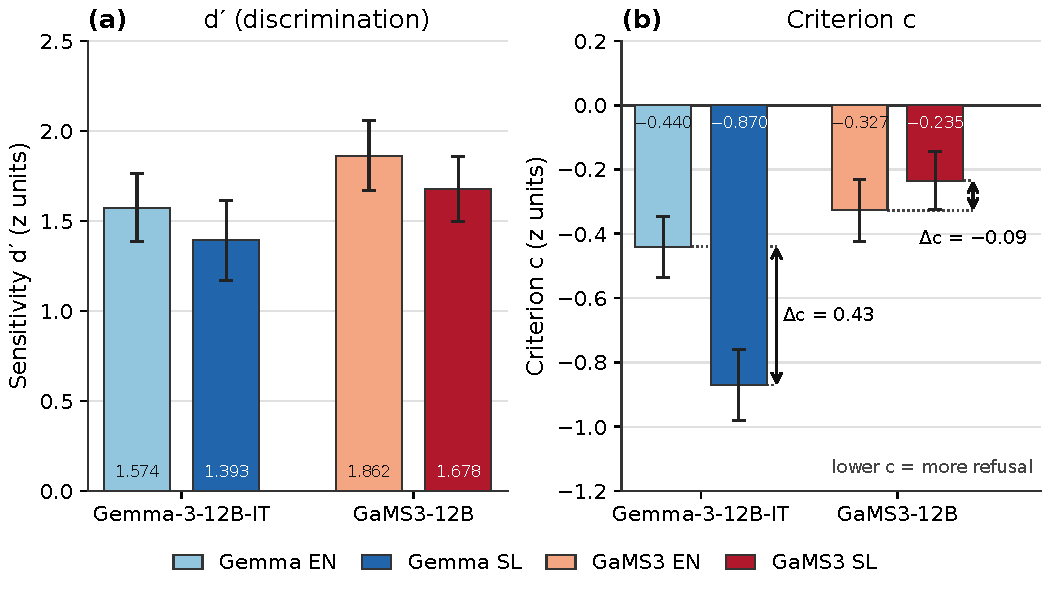
\includegraphics[width=\linewidth,height=0.85\textheight,keepaspectratio]{figures/fig_hard_sdt_v0.pdf}
  \caption{Signal-detection decomposition of refusal on the HARD set (349 unsafe + 1,093 safe items; Experiment~5, Iteration~2). Both models lose similar discrimination in Slovene (DiD $d' = -0.003$). Only Gemma's criterion moves toward refusing: DiD $c = +0.52$ $[0.38, 0.68]$. The criterion contrast depends on the coding rule: when partial answers are coded as refusals, DiD $c$ reverses.}
  \label{fig:hard_sdt}
\end{figure}

This criterion shift is fragile under partial-as-refusal coding, and the DEV gemini judge produced a comparable estimate ($+0.67$). It replicates across OR-Bench items alone ($+0.70$ [0.50, 0.93]) and survives dropping MT-fragile items ($+0.62$ [0.46, 0.79]).


\subsection{Artifact~7: Teacher-Inheritance Screen (Experiment~7)}
\label{gen_art_experiment_7}

Five systems were run on byte-identical prompts: GaMS3-12B-Instruct (NF4), Gemma-3-12B-IT (NF4), Qwen3-235B-A22B (the SFT data generator), Qwen3-14B (same-family positive control, NF4), and Llama-3.3-70B (outgroup placebo).

\subsubsection{Decision Inheritance: Uninterpretable}

The fingerprint-calibration gate failed. The positive control asked whether the instrument can detect within-family resemblance: the Qwen3-14B-to-Qwen3-235B kappa should exceed the Qwen3-14B-to-Gemma kappa by at least 0.10. The observed difference was $-0.001$ [$-0.074, 0.079$]: the instrument cannot distinguish same-family from cross-family agreement.

\subsubsection{Wording Inheritance: Supported}

Refusal wording tells a different story. The SFT-source classifier attributed 95.8\% of GaMS3's English refusal first sentences to the Qwen teacher family.

\begin{table}[!htbp]
\centering
\caption{Refusal first-sentence origin (share found verbatim in SFT data; Experiment~7, Iteration~2).}
\label{tab:wording_exp7}
\begin{tabular}{lcc}
\toprule
Model & EN & SL \\
\midrule
GaMS3-Instruct & 0.761 & 0.908 \\
Gemma-IT & 0.000 & 0.030 \\
Qwen3-235B & 0.757 & 0.015 \\
Qwen3-14B & 0.092 & 0.007 \\
Llama-3.3-70B & 0.254 & 0.016 \\
\bottomrule
\end{tabular}
\end{table}

GaMS3 and the teacher share the same refusal vocabulary to the same degree (76\%), and both are distinct from Gemma (0\%). In Slovene, GaMS3 uses the machine-translated SFT wording (91\%), not the teacher's live Slovene output (1.5\%).

\subsection{Artifact~8: Heretic Transfer-Curve Re-Test (Experiment~8)}
\label{gen_art_experiment_8}

This artifact re-tested the iteration-1 finding using a fresh 200-item RefusEU-TRAIN probe, item-matched across three arms. Both models were run through an identical code path (NF4) over three dose curves: confirmatory curve B (29 paired Heretic trials), lambda-scaling curve, and mean-projection curve.

\textbf{Note:} The primary readout was the unvalidated lexicon (the Llama-3.1-8B judge labelled only 3,374 of 24,000 rows, with kappa 0.52).

\begin{table}[!htbp]
\centering
\caption{$G_3$ across dose curves (Experiment~8, Iteration~2).}
\label{tab:g3_exp8}
\begin{tabularx}{\linewidth}{lXcc}
\toprule
Curve & $G_3$ [95\% CI] & Verdict ($m = 0.675$) & Verdict ($m_{\text{local}} = 0.20$) \\
\midrule
B (29 paired trials) & $-2.36$ [$-3.18, -1.62$] & SL\_OVER\_EXPOSURE & SL\_OVER\_EXPOSURE \\
A1 (lambda scaling) & $-0.19$ [$-1.03, 0.78$] & INCONCLUSIVE & INCONCLUSIVE \\
A2 (mean-projection) & excluded (non-specific) & n/a & n/a \\
\bottomrule
\end{tabularx}
\end{table}

The confirmatory curve confirms and strengthens the iter-1 finding. The lambda-scaling curve gives a much smaller and non-significant intercept: the two curves disagree.

\begin{figure}[!htbp]
  \centering
  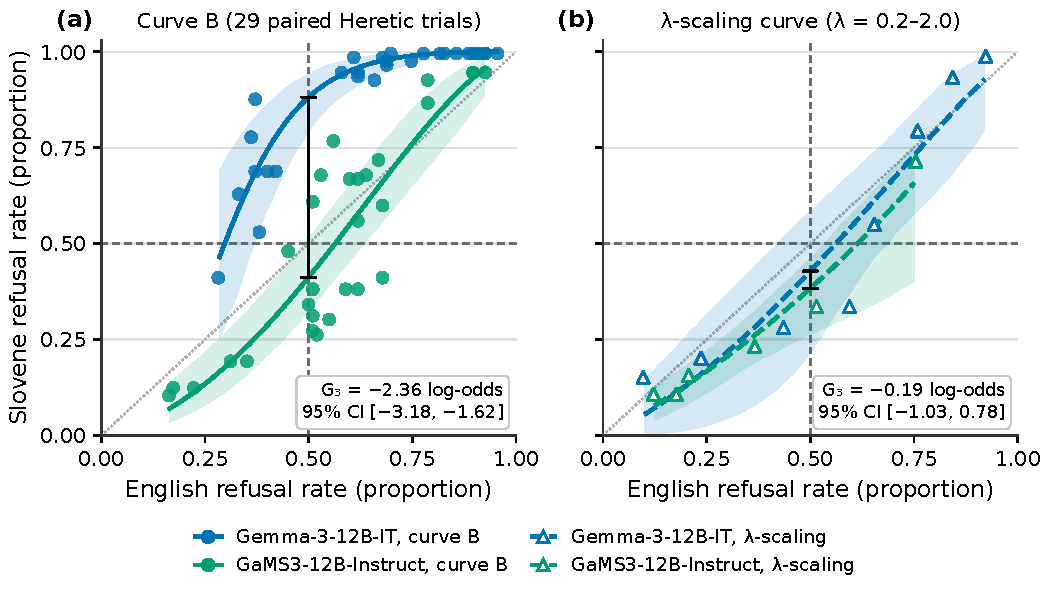
\includegraphics[width=\linewidth,height=0.85\textheight,keepaspectratio]{figures/fig_transfer_retest_v0.pdf}
  \caption{Slovene refusal rate against English refusal rate after Heretic abliteration (Experiment~8, Iteration~2). Filled circles with solid fits: confirmatory curve B ($G_3 = -2.36$ $[-3.18, -1.62]$). Open triangles with dashed fits: lambda-scaling ($G_3 = -0.19$ $[-1.03, 0.78]$). The two curves disagree.}
  \label{fig:transfer_retest}
\end{figure}

\subsection{Artifact~9: Reconciliation of Iteration-1 Findings (Evaluation~1)}
\label{gen_art_evaluation_1}

This \$0 evaluation harmonised all iteration-1 screens onto a single readout.

\textbf{Key finding 1: Prefill cells are unmeasurable.} No readout reached kappa 0.60 on prefill continuations. The prefill-depth signature (alternate~4) and the iter-1 transfer-curve estimate are therefore uncitable.

\textbf{Key finding 2: GaMS3 Slovene deflection.} 34.6\% (115 of 332) of GaMS3's Slovene prefill continuations paraphrased the harmful request back, a pattern absent in all other cells (0\%).

\textbf{Key finding 3: Meta-analysis of the GaMS3 Slovene deficit.} A generalised least-squares meta-analysis gave $-0.50$ [$-0.82, -0.21$]; REML with modified Hartung-Knapp-Sidik-Jonkman correction gave $-0.71$ [$-1.43, 0.00$]; $I^2$ was 0.40.

\begin{table}[!htbp]
\centering
\caption{Reconciliation verdict table (Evaluation~1, Iteration~2).}
\label{tab:reconciliation}
\begin{tabularx}{\linewidth}{llll}
\toprule
Claim & Iter-1 verdict & Harmonised verdict & Changed? \\
\midrule
Main/Alt-1 (D) & INCONCLUSIVE & INCONCLUSIVE & N \\
Alt-2 (base geom.) & DEAD & DEAD & N \\
Alt-3 (persona) & UNTESTABLE & UNTESTABLE & N \\
Alt-4 (prefill) & NOT SURVIVED & UNCITABLE & Y \\
C1 (identity) & PASS (3.22) & PASS (3.22) & N \\
C3 (transfer curve) & FAILS ($-1.86$) & UNCITABLE (prov.\ $-0.44$) & Y \\
C4 (anc.\ induction) & FAILURE BRANCH & FAILURE BRANCH & N \\
C5a (SL KL) & REVERSES ($< 1$) & REVERSES (reprod.) & N \\
C5b (re-selection) & UNPOWERED & UNPOWERED & N \\
\bottomrule
\end{tabularx}
\end{table}

\subsection{Experiment~6: Refusal-Depth Pipeline (Not Scored)}
\label{gen_art_experiment_6}

This artifact produced a Python pipeline for measuring refusal depth across abliteration steps. It defined the experimental protocol and data-flow but produced no scored output.


% ============================================================
\section{Iteration 3}
% ============================================================

\subsection{Strategy}

Three open problems guided this iteration. First, the experiment~8 transfer-curve headline rested on the lexicon and an unvalidated Llama-3.1-8B judge. Second, two mechanistic hypotheses remained untested: whether a geometrically separate ``Slovene caution direction'' exists (M-a), and whether the refusal direction has greater induction potency in Slovene (M-b). Third, no utility control had been run. The iteration ran five artifacts. The OpenRouter budget was exhausted throughout.

\subsection{Artifact~10: Screen Repair of Experiment~8 (Evaluation~2)}
\label{gen_art_evaluation_2}

This evaluation re-judged experiment~8's 24,000 saved responses with Qwen3-14B and Mistral-Small-24B. Qwen3-14B was selected because only it had full coverage (19,971 rows vs 2,614 for Mistral-Small-24B). Calibration kappa was 0.36 overall (EN 0.25), below the archived Llama-3.1-8B's 0.52.

The lexicon finding ($-2.36$) reproduced exactly from the saved response files.

Under the Qwen3-14B judge: the integrated gap was $-1.95$ [$-3.75, -0.78$] under REFUSE-only coding. Under PARTIAL-as-refusal coding, the lag becomes INCONCLUSIVE. The finding is fragile to how partial compliance is classified.

\textbf{Bias tipping analysis.} The Gemma-SL false-REFUSE path is robust, but the GaMS-SL false-COMPLY path is not: $\varepsilon^* = 0.098$ to reach $-m$ (0.143 to reach 0), which requires only a $\sim$10\% error rate.

\begin{table}[!htbp]
\centering
\caption{Judge kappa against blind adjudication on edited rows (Evaluation~2, Iteration~3).}
\label{tab:judge_kappa_eval2}
\begin{tabular}{lc}
\toprule
Instrument & Kappa (binary-R) \\
\midrule
Gemini-2.5-flash & 0.43 \\
Qwen3-14B & 0.26 \\
Llama-3.1-8B & 0.22 \\
Lexicon & 0.20 \\
\bottomrule
\end{tabular}
\end{table}

All instruments are weak on edited rows. The signal is real, but the magnitude is uncertain by at least a factor of two.

\subsection{Artifact~11: Cross-Lingual Abliteration Lag on Fresh Probe (Experiment~9)}
\label{gen_art_experiment_9}

Both models were run in FP8 quantization on a fresh 300-item probe set with 40 paired Heretic trials and a 9-point lambda curve. The primary judge was a DeBERTa classifier distilled from 12,639 archived gemini labels (calibration kappa 0.84).

On the 9-point lambda curve, the transfer-curve intercept was $-0.97$ [$-1.56, -0.44$], exceeding the pre-registered margin ($m = 0.675$). Under Llama-3.1-8B, the intercept was $-1.72$ [$-2.30, -0.96$].

\begin{figure}[!htbp]
  \centering
  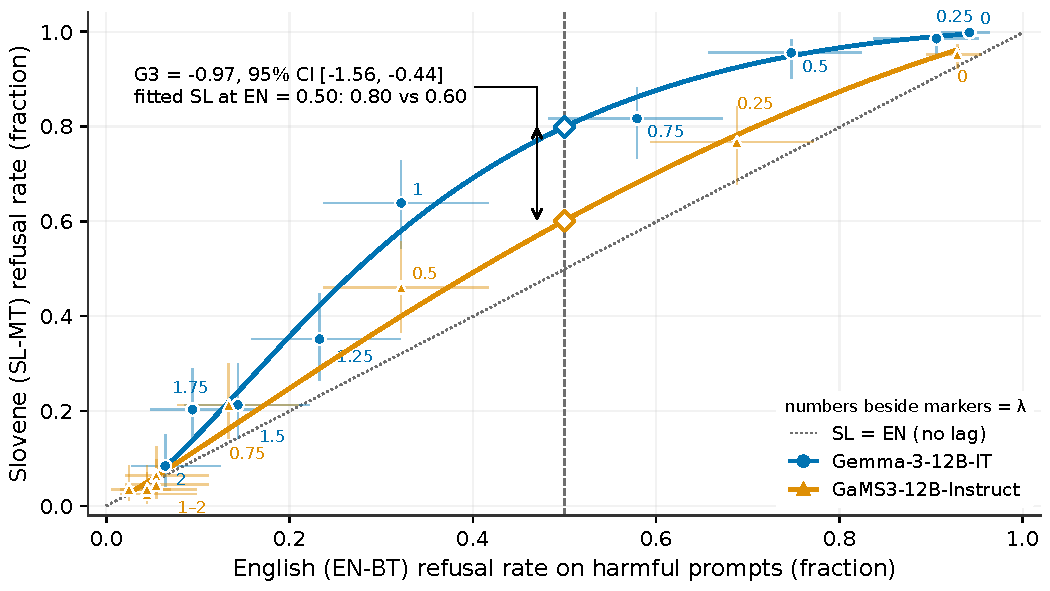
\includegraphics[width=\linewidth,height=0.85\textheight,keepaspectratio]{figures/fig_lambda_exp9_v0.pdf}
  \caption{Slovene refusal rate against English refusal rate across 9 lambda doses (Experiment~9, Iteration~3). The transfer-curve intercept $G_3 = -0.97$ $[-1.56, -0.44]$. The pre-registered support rule is not met.}
  \label{fig:lambda_exp9}
\end{figure}

The paired-trial curve had only 7 trials that passed quality gates, all at high English refusal, and could not identify the intercept.

The engine-equivalence gate failed (NF4-vs-FP8 first-token agreement was 0.86 and 0.88, below 0.90).

\begin{table}[!htbp]
\centering
\caption{Unedited refusal rates on the 300-item fresh probe (DeBERTa judge; Experiment~9, Iteration~3).}
\label{tab:exp9_rates}
\begin{tabular}{lcccc}
\toprule
Model & EN harmful & SL harmful & EN benign & SL benign \\
\midrule
Gemma-IT & 0.94 & 1.00 & 0.08 & 0.26 \\
GaMS3-Instruct & 0.93 & 0.95 & 0.04 & 0.18 \\
\bottomrule
\end{tabular}
\end{table}


\subsection{Artifact~12: Mechanism Test (Experiment~10)}
\label{gen_art_experiment_10}

This experiment tested two mechanistic hypotheses. The judge was a TF-IDF surrogate trained on 11,767 archived gemini labels (kappa 0.68 EN, 0.82 SL).

\subsubsection{Geometry: EN and SL Refusal Directions Are Nearly Collinear}

\begin{table}[!htbp]
\centering
\caption{Geometry of refusal directions at $L^*$ (Experiment~10, Iteration~3).}
\label{tab:geometry_exp10}
\begin{tabular}{lcccc}
\toprule
Model & $\cos(r_{\text{EN}}, r_{\text{SL}})$ & $f$(SL energy in EN dir.) & Ceiling $\cos$ & Perp share \\
\midrule
Gemma-IT & 0.991 & 0.983 & 0.999 & 0.13 \\
GaMS3 & 0.986 & 0.973 & 0.998 & 0.16 \\
\bottomrule
\end{tabular}
\end{table}

At each model's best layer, the refusal directions are nearly collinear. Only 13--16\% of the Slovene refusal signal is perpendicular to English. However, at a common layer the model difference reverses ($f = -0.009$, perp share 0.31 vs 0.38). The geometry result is layer-dependent.

\subsubsection{Induction: The Slovene-Perpendicular Direction Does Not Induce Refusal}

Adding $u_{\text{SLperp}}$ to harmless activations never induced refusal above 50\% in either model. The $u_{\text{SLperp}}$ direction is inert as a refusal inducer.

\textbf{Induction hypothesis: NOT SUPPORTED.}

\subsubsection{Add-On Neutralisation}

At Gemma's selected abliteration strength, the baseline lag was $+1.98$ [1.41, 2.73]. The $u_{\text{SLperp}}$ cut-vs-random difference excluded 0 only at $s=1.5$ (0.62 [0.38, 0.97]) but failed the EN-invariance gate at $-18$ pp EN. Only ablating the full Slovene refusal direction ($A_{\text{SLfull}}$) closed the lag ($-6.17$), at the cost of 50\% degenerate outputs. GaMS Lag($E_0$) $= -0.33$ [$-0.70, 0.07$] fails the add-on precondition, so GaMS add-on results are uninformative.

\subsubsection{G3\textsubscript{op} on the SCREEN Items}

$G3_{\text{op}}$ on the experiment~8 SCREEN items was $-2.30$ [$-3.12, -1.61$], computed as Lag$_{\text{GaMS}}$ minus Lag$_{\text{Gemma}}$ at each model's $E_0$ operating point.


\subsection{Artifact~13: FINAL Confirmation on Reserved Split (Experiment~11)}
\label{gen_art_experiment_11}

Both models were run in NF4 quantization on RefusEU-x FINAL MT pairs (Gemma $n = 200$, GaMS $n = 1{,}101$ EN / 652 SL), plus a 247-item Hungarian arm and the HARD set. The experiment generated 27,264 responses with Qwen3-14B as judge.

The transfer-curve intercept on the 8-step FINAL lambda curve was $-0.60$ [$-1.31, +0.40$], verdict ESTIMATE. Permutation $p = 0.092$.

\begin{table}[!htbp]
\centering
\caption{McNemar rates on the reserved split (Qwen3-14B judge, REFUSE-only; Experiment~11, Iteration~3).}
\label{tab:exp11_rates}
\begin{tabular}{lcccc}
\toprule
Model & EN orig & EN edit & SL orig & SL edit \\
\midrule
Gemma-IT & 0.98 & 0.645 & 0.99 & 0.68 \\
GaMS3-Instruct & 0.97 & 0.58 & 0.97 & 0.46 \\
\bottomrule
\end{tabular}
\end{table}

\begin{table}[!htbp]
\centering
\caption{Belebele accuracy (200 items; Experiment~11, Iteration~3).}
\label{tab:belebele_exp11}
\begin{tabular}{llccc}
\toprule
Model & Condition & EN & SL & HU \\
\midrule
Gemma-IT & Original & 0.930 & 0.885 & 0.880 \\
Gemma-IT & Edit (lam=1) & 0.930 & 0.885 & 0.880 \\
GaMS3-Instruct & Original & 0.905 & 0.875 & 0.870 \\
GaMS3-Instruct & Edit (lam=1) & 0.910 & 0.870 & 0.825 \\
\bottomrule
\end{tabular}
\end{table}

The GEE three-way interaction gams:sl:edit was $+1.06$ ($p = 0.022$). A positive three-way term on a refusal log-odds model means the edit shrinks GaMS3's SL-EN margin \emph{less} than Gemma's. The model difference in SL-EN margin is largely baseline: gams:sl $= -1.73$ ($p = 3\times 10^{-5}$). On FINAL, the model difference in SL-vs-EN refusal is largely pre-edit, not edit-induced.


\subsection{Artifact~14: Utility Control (Experiment~12)}
\label{gen_art_experiment_12}

The utility control used lm-eval on six zero-shot multiple-choice tasks: ARC-Challenge, BoolQ, HellaSwag, OpenBookQA, PIQA, and Winogrande, with 300 paired English/Slovene items per task.

\begin{table}[!htbp]
\centering
\caption{Catastrophe gate (300-item full sets; Experiment~12, Iteration~3).}
\label{tab:catastrophe_exp12}
\begin{tabular}{llccl}
\toprule
Model & Condition & EN loss (95\% hi) & SL loss (95\% hi) & Verdict \\
\midrule
GaMS3 & Iter-1 edit & 0.018 (0.039) & $-0.007$ (0.021) & OK \\
GaMS3 & Art-2 edit & 0.020 (0.043) & 0.009 (0.038) & OK \\
Gemma & Iter-1 edit & $-0.008$ (0.009) & $-0.022$ (0.024) & OK \\
Gemma & Art-2 edit & $-0.016$ (0.002) & $-0.049$ ($-0.000$) & OK \\
\bottomrule
\end{tabular}
\end{table}

\begin{table}[!htbp]
\centering
\caption{Language asymmetry and interaction (Experiment~12, Iteration~3).}
\label{tab:asymmetry_exp12}
\begin{tabular}{llc}
\toprule
Model & Condition & $A = H_{\text{SL}} - H_{\text{EN}}$ [95\% CI] \\
\midrule
GaMS3 & Iter-1 edit & $+0.025$ [$-0.009, 0.060$] \\
GaMS3 & Art-2 edit & $+0.011$ [$-0.023, 0.050$] \\
Gemma & Iter-1 edit & $+0.014$ [$-0.036, 0.082$] \\
Gemma & Art-2 edit & $+0.033$ [$-0.020, 0.125$] \\
\bottomrule
\end{tabular}
\end{table}

The edit does not damage Slovene downstream skills more than English ones. The random-adjusted excess asymmetry excludes zero for GaMS3 ($+0.051$ [$+0.012, +0.093$]). Localised costs include GaMS3's English ARC-Challenge ($3.7$ pp, $p = 0.041$) and BoolQ ($-2.0/-2.3$ pp), both replicating across two edits.

\begin{table}[!htbp]
\centering
\caption{KL footprint (Experiment~12, Iteration~3).}
\label{tab:kl_exp12}
{\small
\begin{tabular}{llcccc}
\toprule
Model & Condition & 1st-tok SL/EN & EXCESS [95\% CI] & 32-tok SL/EN \\
\midrule
GaMS3 & Iter-1 edit & 0.52 & 0.47 [0.38, 0.60] & 0.39 \\
GaMS3 & Art-2 edit & 0.54 & 0.49 [0.40, 0.62] & 0.38 \\
Gemma & Iter-1 edit & 0.72 & 0.63 [0.34, 1.17] & 0.26 \\
Gemma & Art-2 edit & 0.72 & 0.63 [0.34, 1.15] & 0.28 \\
\bottomrule
\end{tabular}
}
\end{table}

Multi-token excess KL ratio: GaMS3 iter-1 0.57 [0.51, 0.66]; Gemma iter-1 0.29 [0.24, 0.37]. The edit touches English distributions more than Slovene.


\subsection{Components Not Executed in Iteration~3}

\begin{table}[!htbp]
\centering
\caption{Iteration-3 components not executed.}
\label{tab:not_exec_iter3}
{\small
\begin{tabularx}{\linewidth}{lXX}
\toprule
Component & Status & Reason \\
\midrule
C-EXT (public abliterated Gemma) & Not generated & Shared cache reclaimed mid-run \\
Frozen-core RQ2 edit & Never ran & All edits are iter-1 reduced-trial NF4 fallback \\
exp10 Qwen3-14B judge & Failed gate & kappa 0.25 EN / 0.33 SL on edited rows \\
exp9 GaMS random-direction control & Not scored & $n_{\text{random\_steps\_scored}} = 0$ \\
exp12 GSM8K & Cut & Budget exhaustion \\
\bottomrule
\end{tabularx}
}
\end{table}


% ============================================================
\section{Iteration 4}
% ============================================================

\subsection{Strategy}

Three problems guided this iteration. First, no artifact's pre-registered verdict reached CONFIRM for the cross-model lag. Second, the mechanism question shifted to M-OUT (output language) vs M-IN (input language). Third, lambda coverage near EN 50\% was sparse. The OpenRouter shared key was available.

Five artifact slots were planned; slot~2 failed. The other four completed.

\subsection{Artifact~15: Readout Completion with Paid Judge (Evaluation~3)}
\label{gen_art_evaluation_3}

This evaluation applied gemini-2.5-flash and gpt-4.1-mini to all saved edited and original rows from experiments~8, 9, 11 and the experiment~10 add-on. Blind adjudication used two Claude-family adjudicators (40-row overlap, inter-adjudicator kappa 0.69).

\subsubsection{Readout Gate: FAILS}

Both decisive cells fail:

\begin{table}[!htbp]
\centering
\caption{Readout gate (gemini-2.5-flash vs adjudication; Evaluation~3, Iteration~4).}
\label{tab:readout_gate_eval3}
\begin{tabular}{lcccc}
\toprule
Cell & Se [95\% CI] & Sp [95\% CI] & $\kappa$ gemini-gpt & Pass \\
\midrule
GaMS-SL-edited & 0.91 [0.74, 0.97] & 0.73 [0.61, 0.83] & 0.39 & False \\
Gemma-SL-edited & 0.99 [0.87, 1.00] & 0.66 [0.43, 0.83] & 0.72 & False \\
\bottomrule
\end{tabular}
\end{table}

The paid judge has high sensitivity but specificity of 0.66--0.73 on edited Slovene rows, below the 0.80 floor.

\subsubsection{Pooled Cross-Model Lag}

\begin{table}[!htbp]
\centering
\caption{Pooled lag estimates (REML + HKSJ, $k = 3$ item bodies, R coding; Evaluation~3, Iteration~4).}
\label{tab:pooled_lag}
\begin{tabular}{lcccc}
\toprule
Readout & $G_3$ [95\% CI] & $G_{3,\text{edit}}$ [95\% CI] & IG [95\% CI] & $I^2$ \\
\midrule
Raw primary & $-1.17$ [$-1.84, -0.50$] & $0.39$ [$-1.95, 2.74$] & $-1.15$ [$-1.31, -0.99$] & 0.22 \\
RG (unstable) & $-1.79$ [$-7.17, 3.58$] & n/a & $-2.02$ [$-5.40, 1.35$] & 0.00 \\
PPI & $-1.77$ [$-1.89, -1.65$] & $0.20$ [$-0.72, 1.11$] & $-2.00$ [$-3.19, -0.82$] & 0.00 \\
TTJ & $-1.10$ [$-4.67, 2.47$] & $0.33$ [$-6.52, 7.18$] & $-1.40$ [$-2.46, -0.33$] & 0.59 \\
\bottomrule
\end{tabular}
\end{table}

The pooled lag is negative under every readout. The edit-induced component is centred near zero in every readout. The lag is entirely explained by the baseline offset: GaMS3 starts with less Slovene refusal than Gemma before any de-censoring. \textbf{R-BASE (baseline offset) is the best-supported account.}

\begin{table}[!htbp]
\centering
\caption{Per-curve $G_3$ decomposition (raw primary readout; Evaluation~3, Iteration~4).}
\label{tab:percurve_eval3}
{\small
\begin{tabular}{lccccc}
\toprule
Curve & $G_3$ [95\% CI] & $G_{3,\text{orig}}$ & $G_{3,\text{edit}}$ & On support & Verdict \\
\midrule
exp9 lambda & $-1.12$ [$-1.70, -0.63$] & $-2.56$ & $1.43$ [0.29, 2.98] & False & ESTIMATE \\
exp11 FINAL & $-1.00$ [$-1.40, -0.68$] & $-1.11$ & $0.10$ [$-0.85, 1.71$] & True & CONFIRM-LAG \\
exp8 A1 & $-1.54$ [$-2.11, -1.00$] & $-1.13$ & $-0.41$ [$-1.65, 1.26$] & False & CONFIRM-LAG \\
exp8 B & $-1.20$ [$-1.77, -0.58$] & $-1.33$ & $0.12$ [$-2.21, 1.47$] & True & ESTIMATE \\
exp10 op point & $-2.42$ & $0.99$ & $-3.40$ [$-6.09, -1.30$] & -- & CONFIRM-LAG \\
\bottomrule
\end{tabular}
}
\end{table}


\subsection{Artifact~16: 2$\times$3$\times$3 Mechanism Test (Experiment~14)}
\label{gen_art_experiment_14}

This experiment crossed input language (EN, SL, HU) with forced output language (EN, SL, HU) at three abliteration doses, for three models: Gemma, GaMS3, and a public abliterated Gemma checkpoint (p-e-w/gemma-3-12b-it-heretic).

\begin{table}[!htbp]
\centering
\caption{Gemma-IT refusal rate per input$\to$output cell, all three doses (Experiment~14, Iteration~4).}
\label{tab:gemma_2x3x3}
{\small
\begin{tabular}{lcccc}
\toprule
Cell & zero & lo ($\lambda=0.5$) & hi ($\lambda=1.0$) & Compliance \\
\midrule
EN$\to$EN & 0.88 & 0.59 & 0.18 & 1.00 \\
EN$\to$SL & 0.95 & 0.92 & 0.77 & 0.99 \\
EN$\to$HU & 0.94 & 0.81 & 0.46 & 0.98 \\
SL$\to$EN & 0.88 & 0.46 & 0.07 & 1.00 \\
SL$\to$SL & 0.95 & 0.85 & 0.56 & 1.00 \\
SL$\to$HU & 0.94 & 0.84 & 0.53 & 1.00 \\
HU$\to$EN & 0.88 & 0.54 & 0.10 & 1.00 \\
HU$\to$SL & 0.95 & 0.93 & 0.83 & 0.96 \\
HU$\to$HU & 0.94 & 0.80 & 0.55 & 1.00 \\
\bottomrule
\end{tabular}
}
\end{table}

\begin{table}[!htbp]
\centering
\caption{GaMS3-Instruct refusal rate per input$\to$output cell, all three doses (Experiment~14, Iteration~4).}
\label{tab:gams_2x3x3}
{\small
\begin{tabular}{lcccc}
\toprule
Cell & zero & lo ($\lambda=0.5$) & hi ($\lambda=0.625$) & Compliance \\
\midrule
EN$\to$EN & 0.82 & 0.30 & 0.21 & 1.00 \\
EN$\to$SL & 0.77 & 0.21 & 0.14 & 0.98 \\
EN$\to$HU & 0.80 & 0.34 & 0.23 & 0.97 \\
SL$\to$EN & 0.87 & 0.25 & 0.16 & 0.00 $\dagger$ \\
SL$\to$SL & 0.87 & 0.20 & 0.15 & 1.00 \\
SL$\to$HU & 0.82 & 0.27 & 0.17 & 0.56 $\dagger$ \\
HU$\to$EN & 0.86 & 0.29 & 0.19 & 0.14 $\dagger$ \\
HU$\to$SL & 0.92 & 0.23 & 0.12 & 0.86 $\dagger$ \\
HU$\to$HU & 0.91 & 0.41 & 0.28 & 1.00 \\
\bottomrule
\end{tabular}
}
\end{table}

Gemma at the high dose shows a large output-language gradient. English-output cells refuse 0.07--0.18 and Slovene-output cells 0.56--0.83. GaMS3 at its high dose spans 0.12--0.28 with no Slovene-output excess. \textbf{GaMS3 did not follow the output-language instruction off the English-input row.} Cells marked $\dagger$ failed the output-language compliance check.

\begin{table}[!htbp]
\centering
\caption{Public checkpoint p-e-w/gemma-3-12b-it-heretic (single external dose; Experiment~14, Iteration~4).}
\label{tab:pew_exp14}
{\small
\begin{tabular}{lccc}
\toprule
Cell & Refusal & Compliance \\
\midrule
EN$\to$EN & 0.05 & 1.00 \\
EN$\to$SL & 0.15 & 0.92 \\
EN$\to$HU & 0.02 & 0.96 \\
SL$\to$EN & 0.01 & 0.99 \\
SL$\to$SL & 0.21 & 1.00 \\
SL$\to$HU & 0.07 & 0.99 \\
HU$\to$EN & 0.04 & 0.94 \\
HU$\to$SL & 0.14 & 0.68 $\dagger$ \\
HU$\to$HU & 0.08 & 1.00 \\
\bottomrule
\end{tabular}
}
\end{table}

\begin{figure}[!htbp]
  \centering
  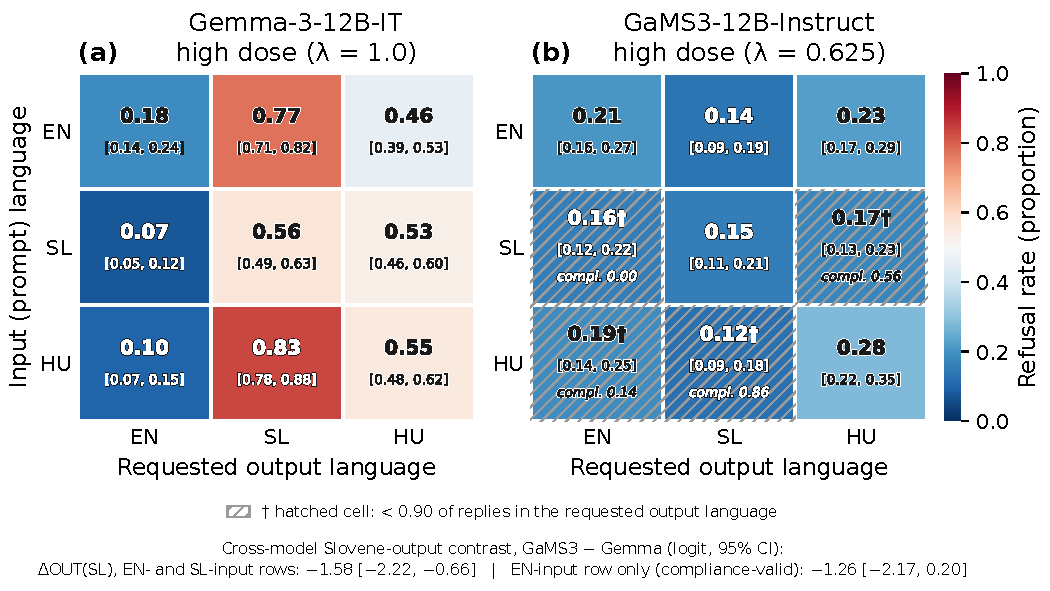
\includegraphics[width=\linewidth,height=0.85\textheight,keepaspectratio]{figures/fig_mechanism_2x3_v0.pdf}
  \caption{Refusal rates of abliterated models on 200 harmful prompts per cell, crossing input language (rows) with output language (columns). Gemma's residual refusal follows the output language; GaMS3 shows no output-language effect. Hatched cells failed the compliance check. On the compliance-valid English-input row, the edit-induced cross-model contrast is $-1.26$ $[-2.17, 0.20]$, including zero.}
  \label{fig:mechanism_2x3}
\end{figure}

\subsubsection{SDT Decomposition}

\begin{table}[!htbp]
\centering
\caption{Signal-detection DiD (Gemma minus GaMS3) at dose zero and $\lambda_{\text{hi}}$ (Experiment~14, Iteration~4).}
\label{tab:sdt_exp14}
\begin{tabular}{llcc}
\toprule
Dose & Contrast & $d'$ DiD & $c$ DiD \\
\midrule
zero & SL output & $-0.13$ [$-0.68, 0.39$] & $-0.76$ [$-1.06, -0.52$] \\
hi & SL output & $0.72$ [$-0.06, 1.30$] & $-1.56$ [$-1.97, -1.29$] \\
zero & SL input & $-0.02$ [$-0.57, 0.58$] & $0.20$ [$-0.07, 0.49$] \\
hi & SL input & $0.27$ [$-0.59, 0.83$] & $0.48$ [0.07, 0.75] \\
\bottomrule
\end{tabular}
\end{table}

The Slovene-output effect sits in the criterion, not in discrimination. The criterion shift is already present before the edit.

\subsubsection{Outcome}

\textbf{Verdict: ESTIMATE (screen).} On the raw readout, edited Gemma's residual refusal follows the output language. The pre-registered raw call is M-OUT SUPPORTED, but the call is not robust across readouts (RG and PPI make no mechanism call; the results file flags robust = False). GaMS3 failed the output-language manipulation off the English-input row.


\subsection{Artifact~17: Fine-Grained Lambda Ladder (Experiment~15)}
\label{gen_art_experiment_15}

This experiment ran a fine-grained lambda ladder on a fresh 300-item RefusEU-TRAIN body disjoint from all prior probes.

\begin{table}[!htbp]
\centering
\caption{Headline $G_3$ decomposition (R coding, raw readout; Experiment~15, Iteration~4).}
\label{tab:g3_exp15}
\begin{tabular}{lccc}
\toprule
Readout & $G_3$ [95\% CI] & $G_{3,\text{orig}}$ [95\% CI] & $G_{3,\text{edit}}$ [95\% CI] \\
\midrule
RAW & $-0.70$ [$-1.01, -0.42$] & $-1.17$ [$-2.83, 0.22$] & $0.47$ [$-0.96, 2.14$] \\
RG & $-0.01$ [$-4.36, 11.27$] & $-1.76$ & $1.75$ \\
PPI & $-0.75$ [$-2.43, 0.99$] & $-1.52$ & $0.76$ \\
TTJ & $-0.79$ [$-1.09, -0.48$] & $-1.37$ & $0.58$ \\
\bottomrule
\end{tabular}
\end{table}

$G_3 = -0.70$ [$-1.01, -0.42$] with MDE 0.42, the most powerful estimate in the entire study. $G_{3,\text{edit}} = +0.47$ [$-0.96, 2.14$]: the edit-induced component spans zero, confirming R-BASE. Curve slopes: $b_{\text{Gemma}} = 0.94$ [0.75, 1.17], $b_{\text{GaMS3}} = 0.80$ [0.63, 0.95]: both near 1, confirming parallel-curve geometry.

\begin{figure}[!htbp]
  \centering
  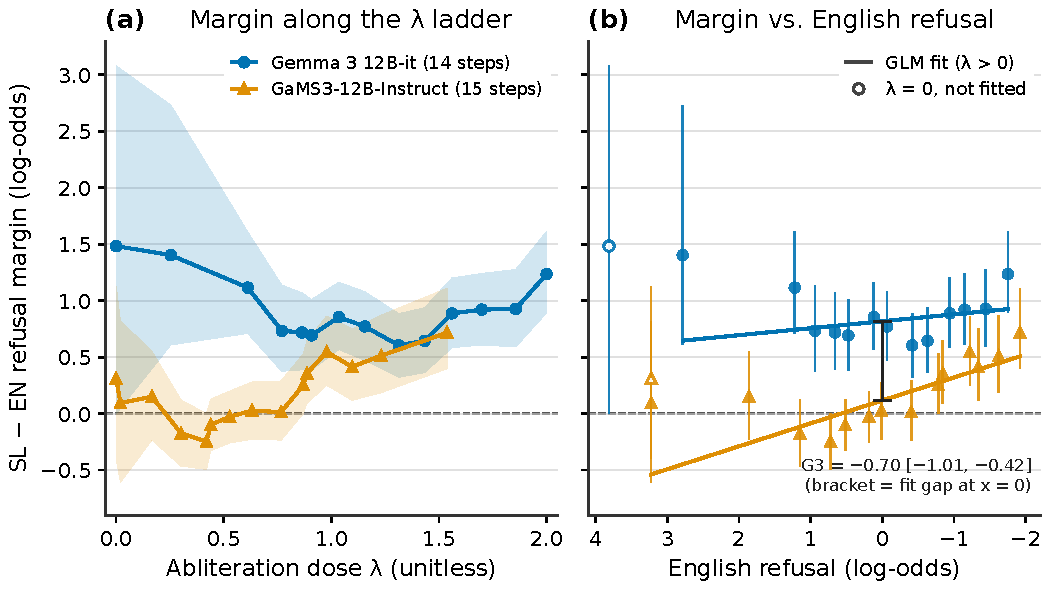
\includegraphics[width=\linewidth,height=0.85\textheight,keepaspectratio]{figures/fig_lambda_ladder_v0.pdf}
  \caption{Slovene-minus-English refusal margin along the fine-grained dose ladder (Experiment~15, Iteration~4). Gemma's margin is positive at every step. GaMS3's margin is near zero in the middle range. $G_3 = -0.70$ $[-1.01, -0.42]$. The edit-induced component spans zero.}
  \label{fig:lambda_ladder}
\end{figure}

\subsection{Artifact~18: Prior-Art and Fact Check (Research)}
\label{gen_art_research_1}

No LLM spend; web greps. \textbf{Novelty:} No published paper crosses prompt language with response language for refusal measurement as of 2026-09-24. The M-IN/M-OUT design is novel (medium confidence).

\subsection{Experiment~13: Held-Out Confirmation (FAILED)}

Approximately 25 minutes into the run, the container lost access to its L4 GPU. The GPU code and the new item body were delivered frozen but untested. The substitute re-readout table (19,195 rows) was frozen but never labelled (the OpenRouter daily key limit was hit at the first call). No number from this artifact appears in any result above.

\begin{table}[!htbp]
\centering
\caption{Experiment~13 judge bake-off (Evaluation~3's 240 adjudicated rows; Iteration~4).}
\label{tab:exp13_bakeoff}
{\small
\begin{tabular}{lccccc}
\toprule
Cell & flash Se & flash Sp & flash $\kappa$ \\
\midrule
GaMS3 EN edited & 0.89 & 0.55 & 0.47 \\
GaMS3 SL edited & 1.00 & 0.47 & 0.57 \\
Gemma EN edited & 0.93 & 0.55 & 0.45 \\
Gemma SL edited & 0.96 & 0.42 & 0.37 \\
Overall ($n = 240$) & 0.95 & 0.50 & 0.47 \\
\bottomrule
\end{tabular}
}
\end{table}

\begin{table}[!htbp]
\centering
\caption{Iteration-4 components not executed.}
\label{tab:not_exec_iter4}
{\small
\begin{tabularx}{\linewidth}{lXl}
\toprule
Component & Status & Reason \\
\midrule
exp13 new Heretic edit & Not executed & GPU lost \\
exp13 held-out confirmation (B-300) & Not executed & GPU lost \\
exp13 random-direction controls & Not executed & GPU lost \\
RQ2 natural RefusEU FINAL under edit & Not executed & GPU lost \\
exp13 paid re-readout (19,195 rows) & Frozen, unlabelled & OpenRouter key limit \\
exp14 ASR readout & One cell only & Not completed \\
\bottomrule
\end{tabularx}
}
\end{table}


% ============================================================
\section{Iteration 5}
% ============================================================

\subsection{Strategy}

Three goals: (i) test the C-OUT finding on a fresh 294-item body with PPI correction (experiment~16); (ii) run the deferred RefusEU FINAL evaluation with 1,300 prompts per cell (experiment~17); (iii) test R-INCAP---whether Gemma's Slovene reserve is real safety or production failure---with StrongREJECT (evaluation~4). Two support artifacts complete the iteration: a paper-number audit (evaluation~5) and a novelty update (research~2).

The experiment~14 mechanism test found that the output-language contrast in Gemma is positive ($+1.14$ [$0.60, 1.56$]) while the input-language contrast is near zero or negative ($-0.60$ [$-1.02, -0.18$]). The compliance-valid cross-model contrast is $-1.26$ [$-2.17, 0.20$], which includes zero. The novelty verdict is downgraded from NOVEL to PARTIALLY OCCUPIED after Addagada~[34] and Nguyen et al.~[35].

\subsection{Artifact~19: C-OUT Test (Experiment~16)}
\label{gen_art_experiment_16}

This experiment tested whether the output-language effect---edited Gemma refusing more when told to write in Slovene than in English---is present on a fresh 294-item body (146 StrongREJECT, 109 HarmBench, 39 JBB) with a new Heretic edit, using PPI as the primary estimator.

\subsubsection{Headline}

The primary PPI estimate is $\text{OUT}_{\text{Gemma}} = +2.43$ [$+0.89, +5.38$] log-odds: edited Gemma refuses 2.43 log-odds more when told to answer in Slovene than in English. The cross-model contrast $\text{dOUT} = -2.31$ [$-5.34, -0.68$] excludes zero. GaMS3 shows no output-language effect: $\text{OUT}_{\text{GaMS3}} = +0.12$ [$-0.47, +0.72$]. The input-language effect in Gemma is negative: $\text{IN}_{\text{Gemma}} = -0.68$ [$-1.23, -0.36$].

All confirmation clauses pass on the consensus reference. However, \textbf{the verdict is capped at ESTIMATE} because the harmful-content adjudication kappa is 0.12 (gate requires 0.60; anchor WEAK).

\begin{table}[!htbp]
\centering
\caption{Primary-judge refusal rates on harmful items, selected cells (Experiment~16, Iteration~5).}
\label{tab:exp16_rates}
{\small
\begin{tabular}{llcc}
\toprule
Model & Cell & Dose & Refusal \\
\midrule
Gemma & EN$\to$EN & hi & 0.330 \\
Gemma & EN$\to$SL & lo & 0.884 \\
Gemma & EN$\to$HU & lo & 0.731 \\
Gemma & SL$\to$EN & lo & 0.344 \\
Gemma & SF\_EN$\to$EN & lo & 0.510 \\
Gemma & SF\_SL$\to$SL & lo & 0.827 \\
Gemma & EN$\to$EN & zero & 0.918 \\
Gemma & EN$\to$SL & zero & 0.969 \\
GaMS3 & EN$\to$EN & hi & 0.490 \\
GaMS3 & EN$\to$SL & hi & 0.449 \\
GaMS3 & EN$\to$EN & zero & 0.820 \\
GaMS3 & EN$\to$SL & zero & 0.786 \\
\bottomrule
\end{tabular}
}
\end{table}

\subsubsection{SDT Decomposition}

\begin{table}[!htbp]
\centering
\caption{Signal-detection DiD at dose zero and dose* (Experiment~16, Iteration~5).}
\label{tab:sdt_exp16}
\begin{tabular}{llcc}
\toprule
Dose & Contrast & $d'$ DiD & $c$ DiD \\
\midrule
zero & SL output & $-0.37$ [$-0.81, 0.07$] & $-0.65$ [$-0.90, -0.46$] \\
lo & SL output & $+0.09$ [$-0.62, 0.57$] & $-1.07$ [$-1.42, -0.85$] \\
\bottomrule
\end{tabular}
\end{table}

The output-language effect sits in the criterion. The criterion shift is already present before the edit and widens under abliteration.

\subsubsection{Benign False Refusal}

Gemma falsely refuses benign prompts more often when told to reply in Slovene (0.38 vs 0.08 on gemini-refused readout). The sign does not hold under all readouts (the template-token judge reverses the cross-model false-refusal difference). Secondary benign verdict: ESTIMATE.

\subsubsection{Public Checkpoint}

The p-e-w/heretic checkpoint shows the same sign: $\text{OUT}_{\text{ext}} = +1.59$ [$+1.10, +2.24$].

\begin{figure}[!htbp]
  \centering
  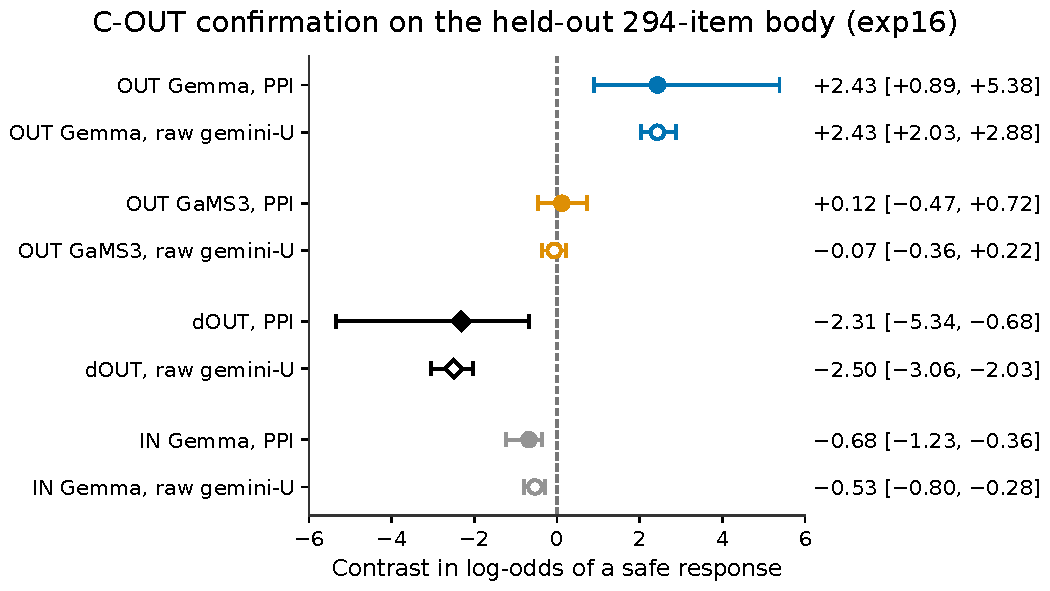
\includegraphics[width=\linewidth,height=0.85\textheight,keepaspectratio]{figures/fig_cout_forest_v0.pdf}
  \caption{C-OUT test (ESTIMATE) on a fresh 294-item body (Experiment~16, Iteration~5). $\text{OUT}_{\text{Gemma}} = +2.43$ [$+0.89, +5.38$] (PPI-corrected). $\text{dOUT} = -2.31$ [$-5.34, -0.68$]. $\text{OUT}_{\text{GaMS3}} = +0.12$ [$-0.47, +0.72$]. All labels are LLM judges and adjudicators, not human; the finding is rated ESTIMATE.}
  \label{fig:cout_forest}
\end{figure}


\subsection{Artifact~20: RefusEU FINAL (Experiment~17)}
\label{gen_art_experiment_17}

This experiment measured what one English-only de-censoring edit buys on RefusEU's own 1,300 prompts per language. The judge stack used local substitutes (PolyGuard, Qwen3Guard, StrongREJECT fine-tuned). 11,600 rows were analysed.

\begin{table}[!htbp]
\centering
\caption{Paired edit effects on RefusEU FINAL (Experiment~17, Iteration~5).}
\label{tab:refuseu_final_exp17}
\begin{tabular}{llcccc}
\toprule
Model & Lang & ASR orig & ASR edit & Delta [95\% CI] & Verdict \\
\midrule
Gemma & EN & 0.045 & 0.897 & 0.852 [0.831, 0.870] & \textbf{ROBUST} \\
Gemma & SL & 0.026 & 0.683 & 0.657 [0.629, 0.683] & \textbf{ROBUST} \\
GaMS3 & EN & 0.033 & 0.970 & 0.937 [0.923, 0.949] & \textbf{ROBUST} \\
GaMS3 & SL & 0.068 & 0.915 & 0.847 [0.826, 0.867] & \textbf{ROBUST} \\
\bottomrule
\end{tabular}
\end{table}

All four cells are ROBUST: the edit produces a massive increase in attack success on RefusEU prompts. The EN-vs-SL within-model difference is not interpretable as a language effect because the prompt sets differ (LaBSE 0.55).


\subsection{Artifact~21: R-INCAP Safety Evaluation (Evaluation~4)}
\label{gen_art_evaluation_4}

This artifact tested whether Gemma's Slovene-output reserve is real safety or production failure. Adjudication used a free LLM panel, NOT human review.

\textbf{At high dose:} the output-language refusal contrast (primary judge) is $\text{OUT}_R = 2.67$ [2.29, 3.12] log-odds and the harmful-content contrast (original StrongREJECT rubric) is $\text{OUT}_U = 2.61$ [2.20, 3.07]. Both are positive and exclude zero. Gemma refuses more in Slovene AND produces less harmful content in Slovene.

\textbf{Verdict: HARMFUL CONTENT SEPARATES (reserve = safety).}

\begin{table}[!htbp]
\centering
\caption{Four-class composition at high dose, decisive cells (Evaluation~4, Iteration~5).}
\label{tab:fourclass_eval4}
\begin{tabular}{lccccc}
\toprule
Cell & $n$ & EXPLICIT & DEFLECT & COMPLY & PF index \\
\midrule
Gemma EN$\to$SL hi & 50 & 0.54 & 0.26 & 0.20 & 0.57 \\
Gemma EN$\to$EN hi & 48 & 0.00 & 0.10 & 0.90 & 0.10 \\
GaMS3 EN$\to$SL hi & 49 & 0.00 & 0.08 & 0.90 & 0.08 \\
GaMS3 EN$\to$EN hi & 50 & 0.00 & 0.12 & 0.88 & 0.12 \\
\bottomrule
\end{tabular}
\end{table}

The production-failure index difference in Gemma is $0.46$ [0.23, 0.65]: half of Gemma's Slovene non-compliance is deflection, consistent with Shen et al.'s relevance curse~[27] and Addagada's output-language effect~[34].

\begin{figure}[!htbp]
  \centering
  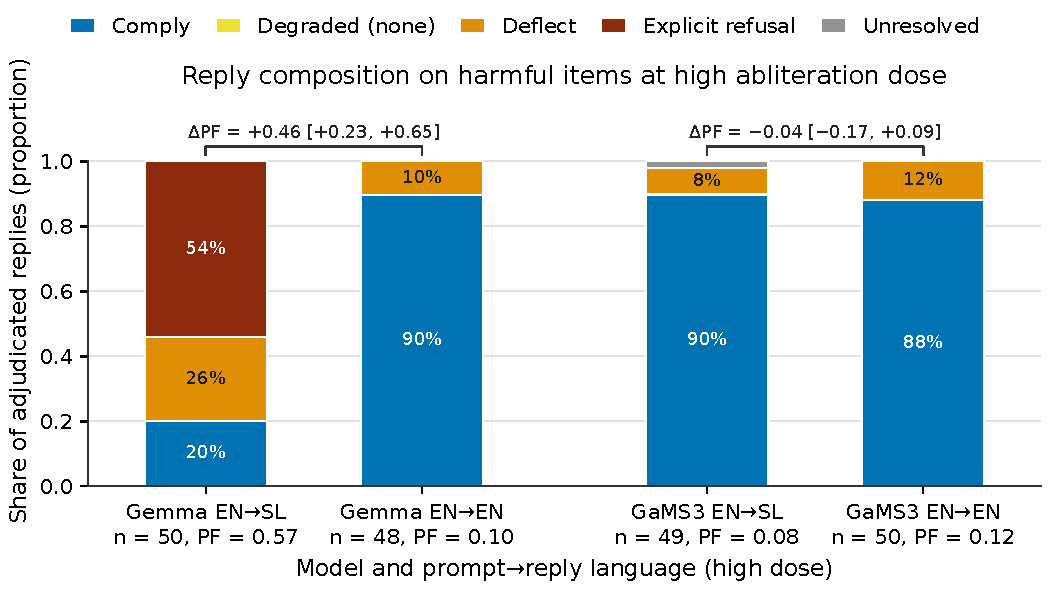
\includegraphics[width=\linewidth,height=0.85\textheight,keepaspectratio]{figures/fig_rincap_composition_v0.pdf}
  \caption{Four-class composition of adjudicated replies at high dose (Evaluation~4, Iteration~5). Gemma EN$\to$SL: 54\% explicit refusal, 26\% deflection, 20\% compliance. Gemma EN$\to$EN: 90\% compliance. PF index difference: Gemma $+0.46$ [0.23, 0.65]; GaMS3 $-0.04$ [$-0.17$, 0.09].}
  \label{fig:rincap_composition}
\end{figure}


\subsection{Artifact~22: Paper Number Audit (Evaluation~5)}
\label{gen_art_evaluation_5}

\textbf{R-BASE ceiling sensitivity.} Experiment~15's baseline component ($-1.17$) is a CEILING-ARTEFACT: one flip in the Gemma lambda-0 Slovene cell (299/300 refusals) moves it inside the margin. Only the experiment~9 lambda body has a ROBUST-OFFSET (fragility index~9).

\textbf{Criterion shift.} The count of 8 of 9 compliance-valid rows with a CI below zero (Gemma's criterion moves toward refusing when it replies in Slovene) was a post-hoc refinement of the analysis, not a pre-registered threshold.

\textbf{Ledger.} 1,176 numeric tokens plus 22 pointer claims: 332 SURVIVE, 844 UNTRACEABLE, 2 REVERSE, 1 SHRINKS.


\subsection{Artifact~23: Novelty and Fact Check (Research~2)}
\label{gen_art_research_2}

\textbf{Main-claim novelty: PARTIALLY OCCUPIED.} Two new preprints partly occupy the lane: Addagada~[34] (forces the output language and finds a relevance curse) and Nguyen et al.~[35] (crosses prompt and response language on benign content). The narrowed design---crossing both factors with safety endpoints on a sibling pair under partial-dose abliteration---remains unoccupied as of 2026-09-25 (medium-low confidence).


\subsection{Iteration-5 Components Not Executed}

\begin{table}[!htbp]
\centering
\caption{Iteration-5 components not executed.}
\label{tab:not_exec_iter5}
{\small
\begin{tabularx}{\linewidth}{lXl}
\toprule
Component & Status & Reason \\
\midrule
exp16 partial-dose points & Not executed & Hard stop at \$4.00 cap \\
exp16 external checkpoints & Not run & Time \\
exp17 primary gemini judge & Replaced by PolyGuard & OpenRouter budget \\
eval4 sonnet-4.5 on low dose & Not run & Budget \\
eval4 human audit & Requested, not performed & No human reviewer \\
Frozen-core Heretic (bf16, 80 trials) & Still not executed & Owed since iteration~1 \\
Natural RefusEU reserved under edit & Still not executed & Owed since iteration~1 \\
\bottomrule
\end{tabularx}
}
\end{table}


% ============================================================
\section{What the Run Learned Overall}
% ============================================================

Five iterations screened the main claim and four alternates against scoring-split data (iteration~1), the reserved evaluation split (iteration~2), fresh data with mechanism tests and utility controls (iteration~3), a paid-judge readout completion with a new mechanism experiment and a fine-grained confirmation (iteration~4), and a C-OUT test with harmful-content endpoints and RefusEU FINAL (iteration~5).

\textbf{Dead alternates.} Two alternates are dead (base-checkpoint geometry and persona gating). A third (prefill-depth signature, alternate~4) is uncitable.

\textbf{Geometry and induction.} The geometry of refusal is layer-dependent: nearly collinear at each model's best layer ($\cos = 0.986$--$0.991$) but divergent at a common layer (perp share 0.31 vs 0.38). The Slovene-perpendicular component does not induce refusal.

\textbf{Teacher inheritance.} GaMS3's refusal \emph{decisions} do not detectably inherit from the Qwen teacher, while its refusal \emph{wording} inherits almost entirely (76\% EN and 91\% SL first sentences verbatim from the SFT data).

\textbf{Primary contest unresolved.} The dose contrast is underpowered across all iterations. The overall GaMS3 Slovene deficit is judge-dependent; the meta-analytic estimate is $-0.50$ [$-0.82, -0.21$\hspace{0pt}].

\textbf{Criterion shift.} On original models and the HARD set, the signal-detection decomposition is robust: the DiD in $d'$ is near zero ($-0.003$), while the DiD in criterion $c$ is $+0.52$ [0.39, 0.67], driven by Gemma over-refusing benign Slovene prompts. The count of 8 of 9 compliance-valid rows with a CI below zero was a post-hoc refinement. The shift is specific to the original-model HARD setting; on edited models (exp11 HARD post-edit), DiD$_c = 0.14$ [$-0.78, 1.12$]: the criterion-shift difference disappears.

\textbf{C-OUT (output-language effect).} Experiment~16 yields OUT$_{\text{Gemma}}(\text{PPI}) = +2.43$ [$+0.89, +5.38$], dOUT $= -2.31$ [$-5.34, -0.68$]; this is an ESTIMATE, not confirmed, because the harmful-content adjudicator kappa is 0.12. The compliance-valid cross-model contrast is $-1.26$ [$-2.17, 0.20$], which includes zero.

\textbf{R-BASE.} The edit-induced component spans zero (experiment~15: $+0.47$ [$-0.96, 2.14$]). The pre-edit baseline is negative everywhere. The curves are parallel. R-BASE (baseline offset) is the best-supported account.

\textbf{R-INCAP.} The reserve is safety, not production failure. Harmful content separates at both doses (OUT$_U$ original rubric $= 2.61$ [2.20, 3.07] at high dose). The four-class decomposition shows that half of Gemma's Slovene non-compliance is deflection (PF index difference 0.46 [0.23, 0.65]).

\textbf{Utility.} The edit does not damage Slovene downstream skills more than English ones. The excess Slovene KL ratio is below~1 in both models across all iterations.

\textbf{RefusEU FINAL.} On 1,300 prompts per cell, the edit is effective in all four cells (ROBUST). The ranking-vs-thresholding analysis shows the guards' AUROC is high but decision thresholds are miscalibrated for Slovene.

\textbf{Novelty.} PARTIALLY OCCUPIED after Addagada~[34] and Nguyen~[35]. The narrowed design remains unoccupied (medium-low confidence).

\section{Open Items}

The readout gate has never passed. The frozen-core Heretic procedure (bf16, 80 trials, Heretic's own selection rule) has never been run. No artifact has scored natural RefusEU reserved-split prompts under the edit. All adjudication is author-LLM, not human. The harmful-content adjudicator kappa (0.12 in experiment~16; 0.59 in evaluation~4) remains below the gate. If R-BASE is correct, the lag is an artefact of model selection (GaMS3 was simply trained to refuse less in Slovene), not a property of the abliteration procedure. The M-OUT finding, rated ESTIMATE as C-OUT, deserves pre-registered confirmation with a validated readout and human adjudication.


% ============================================================
\section{References}
% ============================================================

{\small
\begin{enumerate}
\item A.~Arditi, O.~Obeso, A.~Syed, D.~Paleka, N.~Rimsky, W.~Gurnee, N.~Nanda. ``Refusal in Language Models Is Mediated by a Single Direction.'' NeurIPS 2024.
\item X.~Wang, M.~Wang, Y.~Liu, H.~Sch\"utze, B.~Plank. ``Refusal Direction is Universal Across Safety-Aligned Languages.'' NeurIPS 2025.
\item H.~Du, W.~Li, M.~Cai, K.~Saraipour, Z.~Zhang, H.~Lakkaraju, Y.~Sun, S.~Zhang. ``How Post-Training Reshapes LLMs.'' arXiv 2504.02904, 2025.
\item U.~Shaham, J.~Herzig, R.~Aharoni, I.~Szpektor, R.~Tsarfaty, M.~Eyal. ``Multilingual Instruction Tuning With Just a Pinch of Multilinguality.'' Findings ACL 2024.
\item F.~Joad, M.~Hawasly, S.~Boughorbel, N.~Durrani, H.~Sencar. ``There Is More to Refusal in Large Language Models than a Single Direction.'' arXiv 2602.02132, 2026.
\item V.~Zhong, Q.~Li. ``Refusal Lives Downstream of Persona in Chat Models.'' ICML 2026 MI Workshop.
\item R.~Aziz, I.~A.~Hanif, F.~Koto. ``Low-Resource Safety Failures Are Action Failures, Not Representation Failures.'' arXiv 2606.01196, 2026.
\item A.~Krasnodebska, W.~Kusa, A.~Lipani. ``Multilingual Refusal Alignment for Safer Large Language Models.'' Findings ACL 2026.
\item W.~Hawkins et al. ``The Heterogeneous Safety Impacts of Benign Multilingual Fine-Tuning.'' arXiv 2606.28843, 2026.
\item X.~Li, Z.-X.~Yong, S.~H.~Bach. ``Preference Tuning For Toxicity Mitigation Generalizes Across Languages.'' EMNLP 2024.
\item A.~Upadhyaya, S.~Sikdar. ``When Safety Speaks a Language: A Mechanistic Analysis of Safety-Language Identity Entanglement in LLMs.'' 2026.
\item S.-Y.~Miao et al. ``Who Bridges Safety? Identifying and Targeting Cross-Lingual Shared Safety Pathways.'' 2026.
\item A.~Oppong et al. ``The Illusion of Cross-Lingual Safety in Low-Resource Languages.'' 2026.
\item C.~Kissane, R.~Krzyzanowski, A.~Conmy, N.~Nanda. ``Base LLMs Refuse Too.'' Alignment Forum, 2024.
\item L.~Chua et al. ``Crosslingual Capabilities and Knowledge Barriers in Multilingual Large Language Models.'' arXiv 2406.16135, 2024.
\item X.~He et al. ``TUBA: Cross-Lingual Transferability of Backdoor Attacks in LLMs with Instruction Tuning.'' Findings ACL 2025.
\item Y.~Wu, L.~Ding, L.~Shen, D.~Tao. ``Edit Once, Update Everywhere.'' Findings ACL 2025.
\item G.~Messenger. ``Detecting Safety Training Modification in Language Models via Activation Analysis.'' IEEE Access, 2026.
\item A.~Labunets. ``Refusal geometry reflects refusal training.'' 2026.
\item D.~Vres, T.~Arcon, T.~Petric, D.~Vajda, M.~Robnik-Sikonja, I.~L.~Bajec. ``Building a Strong Instruction Language Model for a Less-Resourced Language.'' arXiv 2603.01691, 2026.
\item R.~Young. ``Comparative Analysis of LLM Abliteration Methods.'' arXiv 2512.13655, 2025.
\item A.~Fafula. ``Abliteration Is Not a Scalpel.'' arXiv 2607.17427, 2026.
\item N.~Truong. ``Abliteration Mitigation via Refusal Aliases.'' arXiv 2608.18093, 2026.
\item P.~E.~Weidmann. ``Heretic: Fully Automatic Censorship Removal for Language Models.'' GitHub, 2025.
\item C.~Lee, T.~Zeng, J.~Jeong, J.~Sohn, K.~Lee. ``How to Correctly Report LLM-as-a-Judge Evaluations.'' ICML 2026.
\item A.~N.~Angelopoulos, J.~C.~Duchi, T.~Zrnic. ``PPI++: Efficient Prediction-Powered Inference.'' arXiv 2311.01453, 2023.
\item L.~Shen, W.~Tan, S.~Chen, Y.~Chen, J.~Zhang, H.~Xu, B.~Zheng, P.~Koehn, D.~Khashabi. ``The Language Barrier: Dissecting Safety Challenges of LLMs in Multilingual Contexts.'' Findings ACL 2024.
\item K.~Y.~Dahir. ``SomaliBench Eval: Measuring English-to-Somali Refusal Gaps.'' arXiv 2605.25420, 2026.
\item M.~Zhang, A.~Patel, S.~T.~Truong, S.~Koyejo. ``Why Do Safety Guardrails Degrade Across Languages?'' arXiv 2605.17173, 2026.
\item C.~Yoon, J.~Park, A.~Ritter. ``Who Pays More for Safety?'' arXiv 2608.22490, 2026.
\item P.~Balani, S.~Panda. ``Hard Negatives Reveal What Easy Negatives Hide.'' arXiv 2609.27758, 2026.
\item R.~P.~Kompella, A.~Mahajan. ``Decided Upstream, Written Late.'' arXiv 2608.08032, 2026.
\item E.~V.~Stein, D.~Meier, T.~Ruas, J.~P.~Wahle, B.~Gipp. ``BabelSteering: Multilingual Safety Alignment via English Steering Vectors.'' arXiv 2608.16577, 2026.
\item T.~C.~Addagada. ``Structural Jailbreaks Generalize but Do Not Compound.'' arXiv 2609.08373, 2026.
\item T.~T.~H.~Nguyen, M.~K.~Tieu, M.~A.~Riegler, P.~Halvorsen, T.~Nguyen. ``Investigating the Influence of Prompt and Response Languages on LLM Content Generation.'' arXiv 2608.26186, 2026.
\item J.~Fiedler. ``Bias and Uncertainty in LLM-as-a-Judge Estimation.'' arXiv 2605.06939, 2026.
\item A.~N.~Angelopoulos, S.~Bates, C.~Fannjiang, M.~I.~Jordan, T.~Zrnic. ``Prediction-Powered Inference.'' Science 382, 669--674, 2023.
\end{enumerate}
}

\end{document}
